\section{Image Filters} \label{s:filters}
	The proper selection of filters is important to the overall effectiveness of the algorithm. As previously mentioned, the intention of DRAGONFIST is to improve a machine learning model's resiliency against adversarial noise. Based on the work done by ------, adversaries can target specific pixels in an image to which noise will be applied. As such, filters which combine the values of pixels with their neighbours are intuitively more desirable as they increase the difficulty of targeting specific areas of the image to which noise will be applied. Therefore, the following filters were considering when designing DRAGONFIST:
	\begin{multicols}{2}
		\begin{itemize}
			\item Edge detection
			\item Gabor
			\item Gaussian
			\item Average rows
			\item Average columns
			\item Average
			\item Rank
			\item Maximum
			\item Minimum
			\item Median
		\end{itemize}
	\end{multicols}

	\subsection{Descriptions} \label{s:filters:descriptions}
		In order to understand what the filters are doing to the images, a brief explanation of each is given.

		\subsubsection{Edge detection} \label{s:filters:descriptions:edgeDetection}
			The edge detection filter uses the Python library \codeword{skimage.filters.sobel} \cite{skikitImageFiltersSobel}. This filter locates and isolates the edges of objects found in an image. An example of this filter applied to an image in the MNIST Fashion database \cite{zalandoresearchFashionMNIST} can be seen in Figure \ref{f:filters:edgeDetection}.
			\begin{figure}
				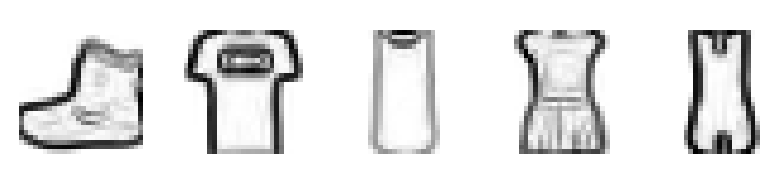
\includegraphics[width=\linewidth]{edge-detection}
				\caption{Edge detection filter on MNIST Fashion image.}
				\label{f:filters:edgeDetection}
			\end{figure}

	\subsection{Filter accuracy} \label{s:filters:accuracy}
		When applying each filter to the system, it is important to remember the overall goal of the model -- to accurately classify its input. Therefore, each filter's accuracy in classification is important to consider to ensure the overall model maintains a high accuracy as well. Each filter was tested individually in order to determine its classification accuracy. The results of these tests can be observed in table \ref{t:filterAccuracies}.
		\begin{table}
			\begin{center}
				\caption{Image filter accuracies.}
				\label{t:filterAccuracies}
				\begin{tabular}{l|l}\hline
					\textbf{Filter} & \textbf{Accuracy}\\\hline
					Edge detection & 90.24\\\hline
					Gabor & 0\\\hline
					Gaussian & 90.07\\\hline
					Average rows & 79.66\\\hline
					Average columns & 82.09\\\hline
					Average & 0\\\hline
					Rank & 88.62\\\hline
					Maximum & 90.07\\\hline
					Minimum & 88.76\\\hline
					Median & 88.62\\\hline
				\end{tabular}
			\end{center}
		\end{table}
